%capitulo02
\label{cap:stateofart}
\noindent 
This section presents our research of the integration platforms under the perspective of the performance of the runtime systems. The technical and scientific literature were reviewed from a set of properties that can have an impact on the performance of runtime system, such properties were classified in two dimensions: efficiency and fairness execution. The dimensions and their respective properties are detailed as follows.

%==============================================================================
\section{Efficiency}
\label{sec:efficiency}
%==============================================================================

This dimension relates to improving the efficiency of the runtime system to process a message, which can also be seen as increasing the average number of messages processed by time unit. It comprises the following properties that relates to the capacity of reducing the real time demanded by the integration solution to completely process a message:
\begin{itemize} 
\item \textbf{Designed for Multi-core}. Multi-core programming has to be carried out in order to take full advantage of multiple cores available in the hardware processors. This property indicates whether the runtime system has been developed to take advantage of multi-core or not. Multiple cores work together to increase the capability of process multiple tasks or increase the performance of the system by operating on multiple instructions simultaneously in an efficient manner. It can take the following values: \texttt{yes} or \texttt{no}. \texttt{yes} indicates the runtime system was developed to take advantage of multi-core hardware, otherwise, the value is \texttt{no}.

\item \textbf{Thread Pool Configuration}. The runtime system allows to configure one or more pools of threads to the integration solution, and this property indicates how threads are managed in these pools. This property may take the following values: \texttt{fixed}, \texttt{limited} or \texttt{elastic}. \texttt{fixed} indicates that a thread pool is composed of a fixed number of threads, which is known at design time; \texttt{limited} indicates the number of threads in a thread pool can increase automatically during runtime until a threshold defined at design time is reached; \texttt{elastic} indicates that the number of threads in a thread pool can automatically increase and decrease during runtime within a range of values defined at design time.
%
\item \textbf{Type of Message Storage in Process}. Messages can contain a huge amount of data, which will have an impact on the amount of memory required by channels inside the integration solution and depending on the type of storage it has an impact on the real time execution. This property indicates whether the message is stored in memory, disk, or both. It may take the following values: \texttt{in memory}, or \texttt{in disk}, or \texttt{in memory \& disk}.
%
\item \textbf{Distributed Process Execution}. Indicates whether an integration solution can be divided and distributed to different machines to execute a set of correlated messages, promoting scalability. This property allows increasing the number of tasks executed per time unit in cases in which there is no dependency between the tasks, i.e., the input data of one task is the output data produced by another task. This property may take the following values: \texttt{yes} or \texttt{no}. \texttt{yes} indicates the runtime system takes advantage of scalability, otherwise, the value is \texttt{no}.
%	
\item \textbf{Thread Pool Creation}. Historical and current execution data can be used by runtime systems to make decisions during runtime, determining optimised strategies to create threads. This property indicates the way and stage at which thread pools can be created. This property may take the following values: \texttt{dynamic} or \texttt{static}. \texttt{dynamic} indicates that thread pool creation is done at runtime from data taken from the runtime system and indicates the need for a pool and \texttt{static} value indicates that the pool creation is done at design time by the software engineer.	
\end{itemize}
%
%==============================================================================
\section{Fairness execution}
\label{sec:fairness}
%==============================================================================

This dimension concerns to assignment of threads to tasks aiming at a fair execution of them to help to minimise the average time that a message takes to be processed in the integration solution. The following properties provide means that contribute to have a fair execution of tasks:
\begin{itemize}
% 	\item \textbf{Priority to task execution}. Indicates whether the runtime system allows tasks to have priority associated with them so that it affects the execution policy by the runtime system. This property may take the following values: \texttt{yes} or \texttt{no}. \texttt{yes} indicates the runtime system can deal with priority in tasks.
%	
\item \textbf{Starvation Detection}. Indicates whether the runtime system is endowed with the capacity to detect tasks that do not execute within an accepted time-frame. This property may take the following values: \texttt{yes} or \texttt{no}. \texttt{yes} indicates the runtime system can detect starvation, otherwise, the value is \texttt{no}. 
%	
\item \textbf{Thread Pool Policy}. Indicates the strategy followed by the runtime system to assign the existing threads to the different tasks. This property may take the following values: \texttt{FIFO}, \texttt{priority} or \texttt{mapping}. \texttt{FIFO} means that the runtime system follows First-In-First-Out(FIFO) heuristic, in which the threads are being allocated the tasks in order that arrive, so that the first ones that arrive are attended to before; \texttt{priority} means that the runtime system allows tasks to have priority associated; and, \texttt{mapping} means that the scheduling policy follows a mapping based on a mathematical model or optimization method that allows finding an optimal scheduling policy by previously evaluating the integration solution.
%	
\item \textbf{Task Complexity}. Indicates whether the runtime system takes into consideration the computational complexity of tasks to allocate threads. This property may take the following values: \texttt{yes} or \texttt{no}. \texttt{yes} indicates that the runtime system knows the computational complexity of each of the tasks and this can be utilised in the decision in choosing the order of execution of tasks, such as tasks of less computational complexity can be executed first, as soon as possible; otherwise, the value is \texttt{no}.
%
\item \textbf{Execution Model}. Indicates the execution model implemented by the runtime system, which deals with the granularity of the execution of tasks. This property may take the following values: \texttt{process-based}, \texttt{task-based} or \texttt{hybrid}. In the \texttt{process-based} model, the runtime system controls process instances as a whole, i.e., there are no means that it can interact with the internal tasks; contrarily, in the \texttt{task-based} model, the runtime system may control both process instances and their internal tasks. In the \texttt{hybrid} model, the runtime system will adopt the model that better fits the execution profile about some predefined parameters, such as message input rate, the number of processors, average message size. 
%
\item \textbf{Throttling Controller}. Indicates whether the runtime system allows controlling the rate of incoming messages on input ports. If the input rate exceeds the processing capacity of the initial tasks, the runtime system can adopt suitable policies, such as, refusing new messages on passive ports or tuning the frequency of the pooling in the active ports. This property may take the following values: \texttt{yes} or \texttt{no}. \texttt{yes} indicates that the runtime system can control the rate of incoming messages, that is, it has a throttling controller; otherwise, the value is \texttt{no}. 
\end{itemize}
%==============================================================================
\section{Analysis and Discussion}
\label{sec:analysis}
%==============================================================================

We selection some popular integration platforms to analyse the values of the described proprieties. For this, we rely in the methodology the integrative literature review, which includes the following steps: identification of the theme and elaboration of the inclusion and exclusion criteria of articles, construction of an instrument for collection of relevant data of the articles found, evaluation and analysis of the articles selected in the research, interpretation and discussion of the results obtained and presentation of the review.

We search the databases: IEEE Xplore, ACM Digital Library, Scorpus, using the keywords: "runtime system" and "execution engine". The inclusion criteria were: articles published in English, abstracts available in the chosen databases, availability of the same in full, published between the period from 2012 to 2017, not to restrict the area of knowledge used by the runtime systems.
We revised the Gartner report~\cite{gartner2016,guttridge2017} and Ovum report~\cite{sharma2017} for integration platforms and also made an exhausting search on the Web to build a list of candidate integration platforms. 

We have adopted the following criteria to select the integration platforms: they must follow the pipes-and-filters architectural style~\cite{alexander1977} and support enterprise integration patterns (EIPs)~\cite{hohpe2004}.
%and have their code under an open source license. 
The pipes-and-filters architecture style suggests dividing a task into smaller tasks, which are connected through communication channels in the message flow of the application, and the output of one task is the input to the next. In this architectural style, the computational components that perform an atomic task on inbound messages to route, transform or modify them and produce one or more outbound messages which are sent to the next filter by means of a communication channel, called pipe. We apply the aforementioned criteria and then we exclude those that did not meet the criteria or had not enough documentation to infer the values of the properties.

Enterprise integration patterns are conceptual standards identified and documented by Hohpe and Woolf~\cite{hohpe2004}, such standards have become a benchmark amongst software engineers and have inspired several integration platforms~\cite{isen2010,dossot2014,fisher2012,frantz2012}. EIPs document a set of best-practices to implement tasks which help to solve recurrent application integration problems.

We have analysed the runtime system of Mule~\cite{dossot2014}, Camel~\cite{isen2010}, Spring Integration~\cite{fisher2012}, Synapse~\cite{rademakers2008,jayasinghe2011}, Fuse~\cite{russell2012}, ServiceMix~\cite{konsek2013}, Petals ESB~\cite{surhone2010}, Jitterbit~\cite{russell2012_1} and WSO2 ESB~\cite{indrasiri2016}. It is important to note that the component SE Camel embeds the Apache Camel routing runtime system to execute enterprise integration patterns (EIP) in Fuse, ServiceMix and Petals, therefore, some properties have the same values.

The comparison of the runtime systems, regarding proprieties related to efficiency and fairness execution are summarised in Table~\ref{tab:comparison}.
\begin{table*}[htbp]
	\centering
	\caption{Comparison between runtime systems.}
    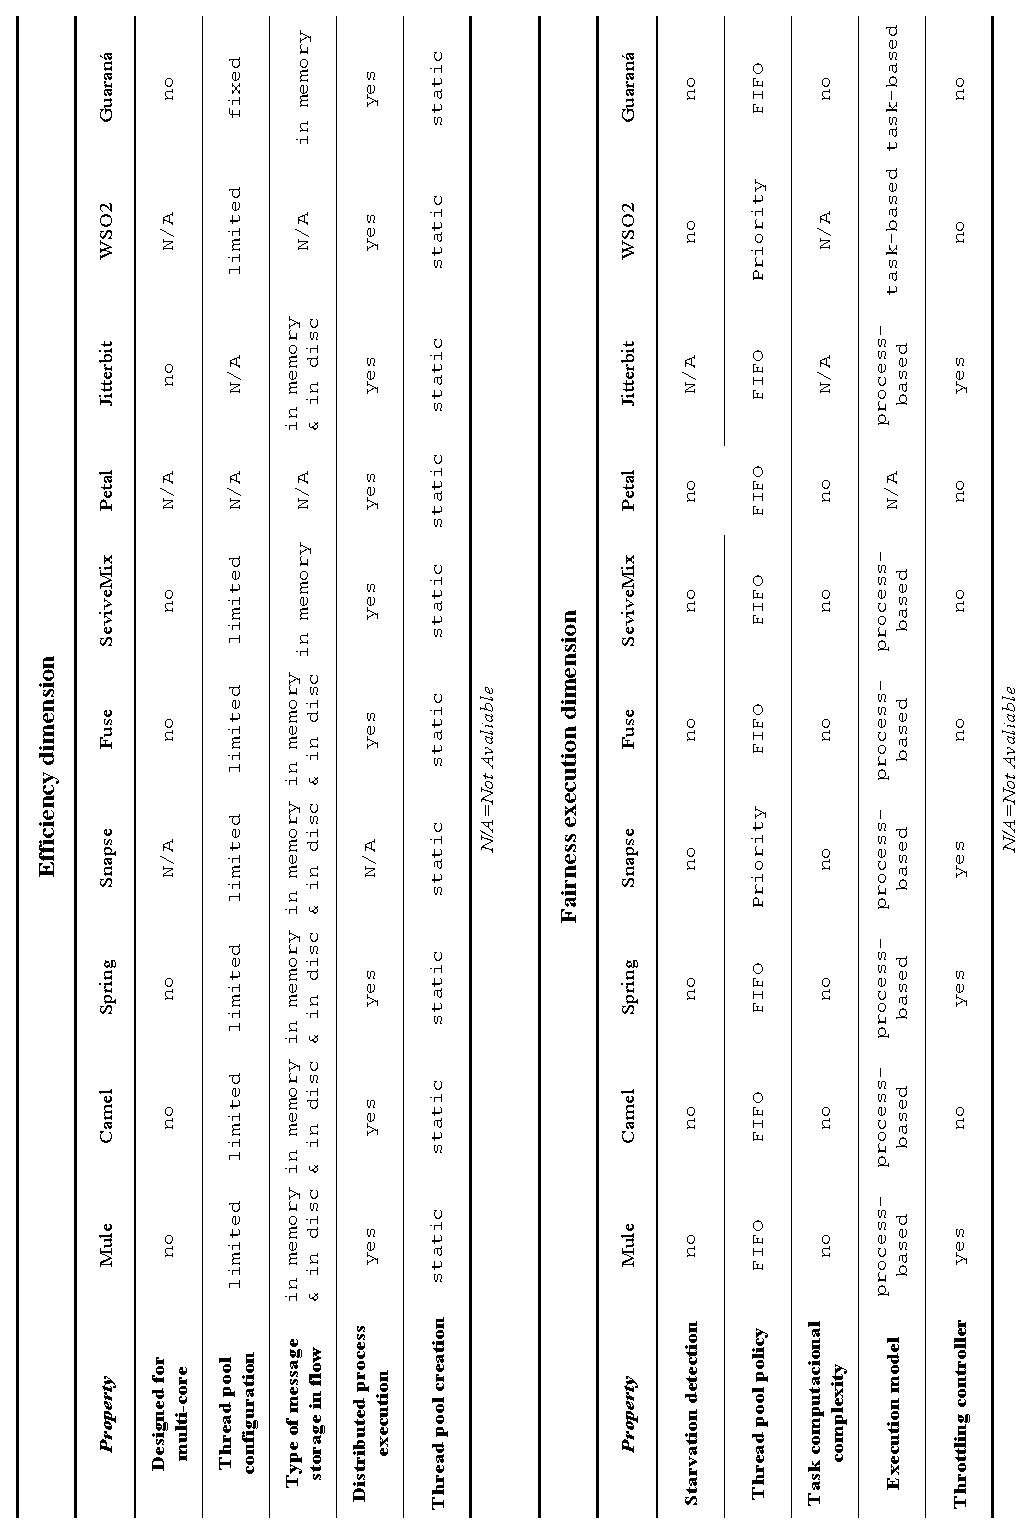
\includegraphics[scale=0.8]{./figs/table_dimensions_v.eps}
	%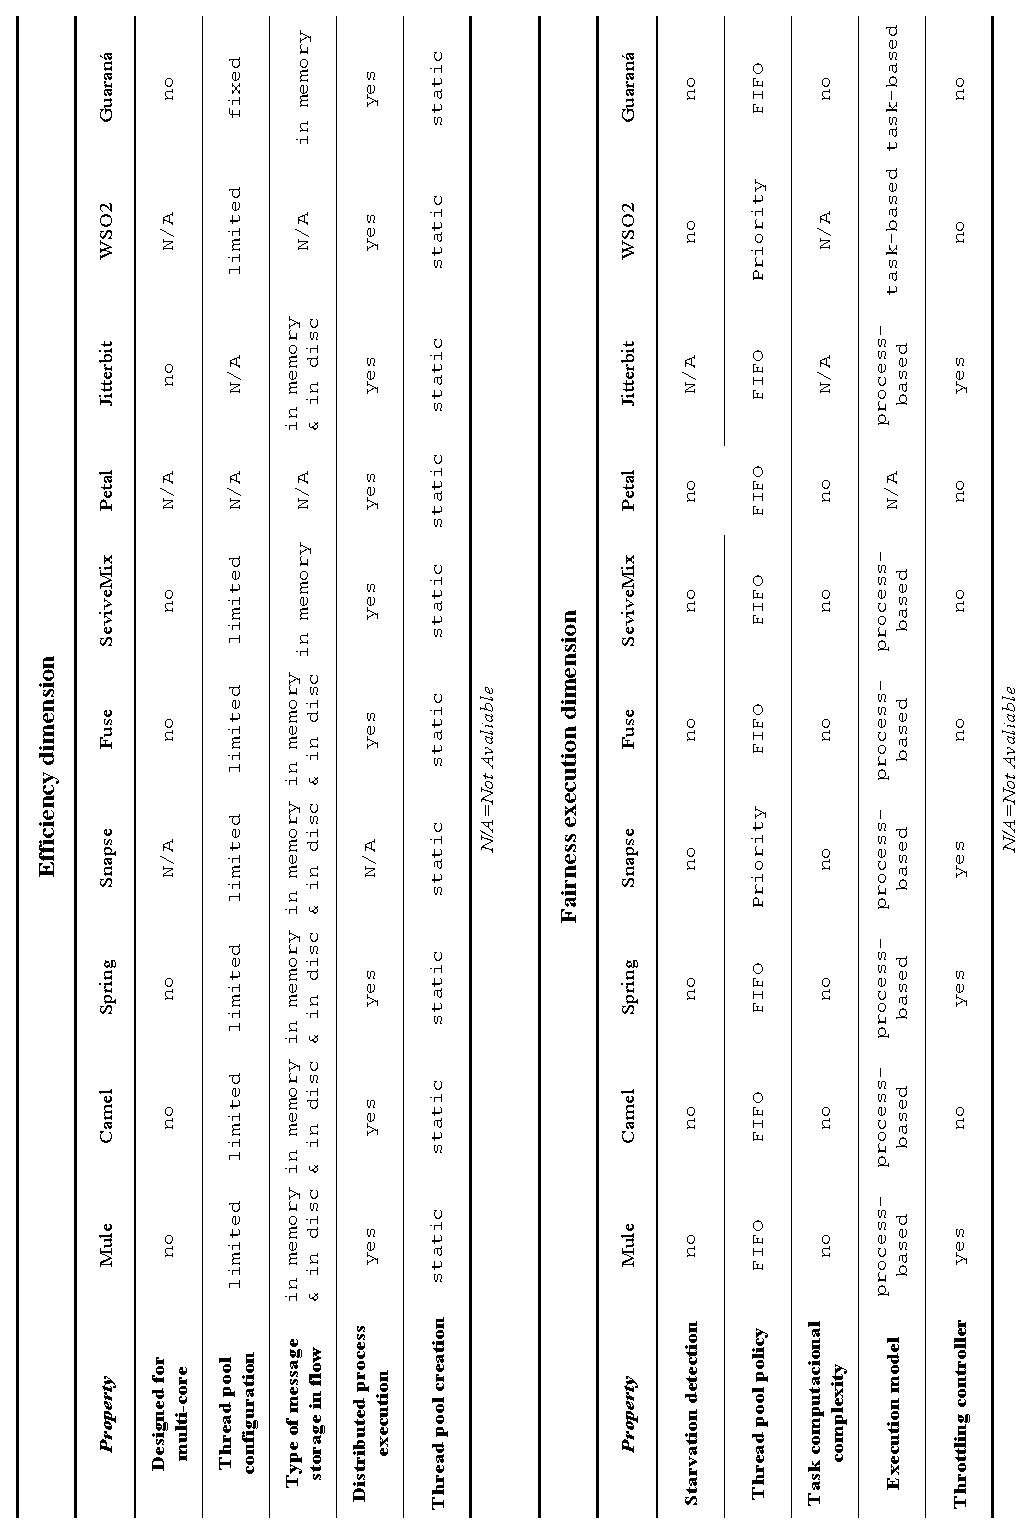
\includegraphics[width=\linewidth]{./figs/table_dimensions_v.eps}
	\label{tab:comparison}
\end{table*}

None of the integration platforms have their runtime system designed to take advantage of multi-core. Although, Mule, Camel and Jitterbit use some language resource for to implement the parallel programming, there not is information about proprieties of runtime systems that take advantage of physically tasks of an integration solution.

Every runtime systems have pools of threads which can increase or decrease the limited number of threads available to tasks, except Petals and Jitterbit, in which there is no information that allow us to evaluate them regarding this property; and Guaraná the provide a fixed pool of threads.

Mule, Camel, Spring Integration, Synapse, Fuse, ServiceMix and Jitterbit can deal with both common data, storing in memory, and big data, storing in disc. ServiceMix and WSO2, there is no information that allow us to evaluate them regarding this property, so we have assumed they, as well as Guaraná, store message only in memory.

The ability to distribute the execution of tasks amongst several virtual machines is present in every analysed runtime systems, except in Synapse, where there is no information that allow us to evaluate them regarding this property. 

None of these runtime systems is able to creation dynamically thread pool, optimising their task execution strategies from the analysis of the flow of messages in the integration solution. Petals, there is no information that allow us to evaluate it regarding this property, so we have assumed it do not provides creation dynamic thread pool.

The capacity to detect tasks that are not executed within an accepted time frame is absent in every analysed runtime systems, except for Jitterbit, there is no information that allow us to evaluate it regarding this starvation detection property. Every analysed runtime systems chose FIFO heuristic as strategy for tasks scheduling, except Synapse and WSO2 have a strategy for distinguish tasks, in order to influence their scheduling, that is, priority based. 

None runtime systems considers the computational complexity of tasks to allocate threads, except for Jitterbit and WSO2, there is no information that allow us to evaluate them regarding this property, so we have assumed they not have considering the computational complexity of tasks to allocate threads.

Every runtime system implement process-based execution model, in which the runtime system controls process instances as a whole, except Guaraná and WSO2 which implement task-based execution model; and Petals, there is no information that allow us to evaluate them regarding this property, so we have assumed they adopt process-based execution model. 

Mule, Spring, Synapse and Jitterbit allow to control the rate of incoming messages on incoming ports; the others have not throttling controller.

Mule, Camel and Jitterbit platforms present resources of parallel programming, but none of the analysed runtime systems are designed to take advantage of the physical cores of the processor.
Runtime systems are similar about pool threads configuration at tasks, however, none has the ability which allows runtime systems automatically increase and decrease to more efficiently meet demand peaks, as well as eliminate threads to release computational resources when they are no more necessary. 

In Mule, the threading profile specifies how the thread pools behave. It is possible to specify a separate threading profile for each input thread pool, flow thread pool, and output thread pool~\cite{Mule}. Camel and ServiceMix offer both a fine grained configuration where it is possible tweak individual pools and have more coarse grained configuration with fall back to global settings; furthermore, it should be possible to define a set of rules which matches, which thread pool a given source should use, task or group of task~\cite{Camel}. Every runtime system has classes which extends a class \texttt{ThreadPoolExecutor} of the language Java and their methods which set size pool, number maximum of thread in pool, amongst others. Camel and ServiceMix allow global settings pools, while Synapse and WSO2 have a property file, which contains global parameters for tuning its global pool of threads~\cite{WSO2}. 

Runtime systems are advanced in storing messages in flow. The ability of disk storage allows runtime systems to deal with big data~\cite{chen2014}, that is, larger data in size or volume. Usually, disk storage can increase the total time of message execution, so that it should be used in scenarios where this type of storage is really needed. Mule uses object stores to persist data for eventual retrieval. Internally, it uses object stores in various filters, routers, and other message processors that need to store state between messages. In most cases, Mule creates and manages object stores automatically, and provides two types of object stores: \texttt{In-memory store} and \texttt{Persistent store}. \texttt{In-memory store} are stores objects in local Mule runtime memory. Objects are lost on shut-down of Mule runtime. In \texttt{Persistent store}, Mule persists data when an object store is explicitly configured to be persistent. In a standalone Mule runtime, Mule creates a default persistent store in the file system~\cite{Mule}. 

Camel and ServiceMix allow to save the message in a persistent store: in a file or database~\cite{isen2010}. Spring Integration defines the \texttt{Message Store} pattern, which allows enterprise integration patterns (EIP) components to store messages typically in some type of persistent store, in addition to capability to buffer messages~\cite{Spring}. Synapse uses the Java classes: \texttt{AbstractMessageStore} and \texttt{InMemoryMessageStore} to store message in disc and in memory, respectively~\cite{Snapse}. Fuse offers a number of different persistence mechanisms besides the default message store, including: \texttt{KahaDB message store}, \texttt{distributed KahaDB}, \texttt{LevelDB} and \texttt{JDBC adapter}. The \emph{KahaDB Message Store} is the default message store uses a hybrid system that couples a transactional journal for message storage and a reference store for quick retrieval. The \texttt{distributed KahaDB} persistence adapter allows to distribute a destinations of broker across multiple \texttt{KahaDB message stores}. The \texttt{LevelDB message} store is a file based message store implemented using LevelDB of Google library to maintain indexes into log files holding the messages. Fuse supports the use of relational databases as a message store through JDBC, where it is possible persistence adapter either coupled with a high performance journal or standalone~\cite{Fuse}. Jitterbit is also able persist message to a file system~\cite{Jitterbit}.

Runtime systems are fit the cloud computing~\cite{hwang2013} environment in which processing can be distributed across multiple virtual machines, providing greater processing power for tasks that can be processed in parallel. However, it is important that the data transfer time from one machine to another minimises the total message processing time because if the total processing time increases, the distributed processing will be detrimental to the performance of the runtime system.

Mule has a virtual server composed of multiple nodes, which ensures high system availability, realising distributed process execution. To get high performance, it is possible configure a Mule cluster or an individual application for maximum performance using a performance profile. By implementing the performance profile for specific applications within a cluster, it is possible maximise the scalability of the deployments while deploying applications with different performance and reliability requirements in the same cluster~\cite{Mule}.

Camel, Fuse and ServiceMix propose different solutions to allow their solution to be scalable, to distribute the load between different instances, such as load balancing, clustering and cloud computing. The approach of the load balancing allows to distribute the load between different endpoints, which plays the role of a \textit{proxy}. The clustering can be achieved through work distribution, consumer competition, amongst others, depending of the infrastructure configuration: one or several instances running on the same machine or distribute across a cloud of servers. For cloud computing, it is possible to create a Cassandra endpoint to allow to consume or to push messages from Cassandra NOSQL database~\cite{Camel}. 

Spring Integration provides a consistent model for intraprocess and interprocess messaging implemented using Java Message Service(JMS)~\cite{fisher2012}. Petals distributes its processes in a static and dynamic way. In static, no new node can be added to a running Petals cluster. In dynamic, it is possible this distribution be updated regularly, so can add new nodes to a running Petals cluster~\cite{Petals}. Jitterbit includes a multi-tenant, auto-scaling agent group called \texttt{Jitterbit Cloud Agent Group}. Agent Groups provide for high availability and load balancing of integration operations across runtime servers within a group. In case of the \texttt{Cloud Agent Group}, it is automatically scaled within the cloud as necessary, and does not require adding runtime servers to expand capacity~\cite{Jitterbit}. 

WSO2 implements a distributed process by means of two models. The first model consists of two sub cluster domains as worker domain and management domain. These sub domains take up load according to a defined load balancing algorithm and auto-scales according to the load on its nodes. The second model consists of a single cluster, where a selected node works as both a worker and a manager. This worker node requires two load balancers and configured in read/write mode, the others are set up in read-only mode. The management node also should be a well-known member in the non-management worker nodes so that state replication and cluster messaging works~\cite{WSO2}.

Analysed runtime systems do not made progress on creating plans that best perform their flows based on statistics or optimization techniques that are being increased performance. The value for the measure used to create such plans came from the monitoring or processing algorithms and usually increase the total processing time. Thus, the plans generated must be good enough to compensate for an initial loss of performance and allow thread pool creation according the demand.

We observe that every runtime systems has some kind of monitoring that allows detect bottlenecks at runtime. Mule can use the management console to monitor the health of a server, see which flows are running or stopped, and determine memory usage. It is possible to view detail information about this server, including deployed applications, alerts, memory usage, plus information about threads, pools, files, server properties, operational system resources, Java Management Extensions (JMX), and server settings~\cite{Mule}. 

Camel has extensive support for JMX to allow monitoring and controlling the Camel managed objects with a JMX client~\cite{Camel}. Spring Integration allows enable \texttt{MessageSource}, \texttt{MessageChannel} and \textit{MessageHandler} metrics, which can indicates bottlenecks. \texttt{MessageSource} only maintains counts, such as number of failed sends, that is, either throwing an exception or rejected by the channel; mean send rate; amongst others. \texttt{MessageChannel} and \texttt{MessageHandler} maintain duration statistics in addition to counts, such as count of messages that are currently buffered by queue, number of currently active threads currently, average of the method execution time over roughly the last ten measurements, amongst others. The time-based metrics which are calculated in real time, and the statistics are calculated when retrieved instead. At runtime, counts and statistics can be obtained. In addition to metrics, it is possible control debug logging in the main message flow.~\cite{Spring}. 

Synapse, Fuse and WSO2 ESB utilise JMX monitoring and management, which allows monitoring of elements that may be indicative of bottlenecks, such as memory allocation, thread utilization, data input and output operations, CPU consumption, and request processing time~\cite{Snapse,Fuse}. Jitterbit provides an interface that let to monitor every integration process and errors; however, the documentation of this platform does not specify which metrics are provided~\cite{Jitterbit}. In case of Petals, many metrics are provided through the Petals CDK, such as current, maximum and minimum number of active threads, response times of the task, and durations of the tasks, amongst others~\cite{Petals}. 

From the analysis of the properties that may have an impact on the efficiency of the runtime systems, we observe that Mule, Camel and Jitterbit are advancing about the programming parallel, although none have actually benefited from multi-core programming. The majority of them already manages the threads, but does not provide the elasticity, which sizes these resources proportionally to their demand in runtime. Most are already able to deal with large volumes of data, because they include features to store data in disk forecasting. Also, they have advanced the issue of exploiting the benefits of distributed processing, because every runtime system has the ability to distribute the execution of tasks amongst several virtual machines. However, they have not yet deepened in the approach of generating execution plans that allow optimising the performance of the runtime system.

In most cases, the runtime system makes no guarantee about the sequence for the execution of the tasks waiting into queue to be attributed to a pool thread. This means that, there is a theoretical risk that a task remains waiting forever to have a thread assigned to it. One possibility would be to monitor the time a task waits to run. However, we did not find metrics in platforms with a similar purpose that allowed the detection of \textit{starvation}.

Every runtime systems adopts heuristics as a scheduling policy to tasks, the default policy enforces \textit{first-in, first-out} ordering, the \textit{priority based} is an alternative implementation that allows messages to be ordered within the channel based upon a priority. Synapse cite also \textit{last-in-first-out} as one of the alternatives~\cite{Snapse1}. For to prioritize to task execution, Synapse e WSO2 uses the class \texttt{PriorityExecutor} do Java, which can be used to execute sequences of tasks with a given priority. This allows software engineer control the resources allocated to executing sequences and prevent high priority messages from getting delayed and dropped~\cite{WSO2}. Class \texttt{PriorityExecutor} is backed by a \texttt{BlockingQueue} and a \texttt{ThreadPoolExecutor}. \texttt{BlockingQueue} is a custom implementation which has multiple internal queues for handling separate priorities. This policy impacting the total processing time of a message. So it is possible give a high priority to tasks which necessity to be to be executed first or more frequently, avoiding they wait in the queue for a time larger than necessary, before to be assign to threads.

Every runtime system is not yet able to know the computational complexity of tasks and neither consider this information to improve its performance. About execution model, the literature shows that the task-based model offers better performance with a steady stream of data input and lower performance when that input rate increases~\cite{frantz2011}. However, except Guaraná and WSO2, most of the runtime systems adopts the execution model process-based, chiefly due to the complexity of the task-based model to provide transaction and fault-tolerance support~\cite{frantz2012}. 

When the message input flow is high, initial tasks tends to accumulate into ready tasks queue, and consequently, ones are more often executed than the other tasks present in the queue. Thus, the throttling controller could avoid can help ensure fairer execution. In Mule, it is possible to arrange for a tasks to actively call a resource at regular intervals, by means of the interface \texttt{Poll scope}~\cite{Mule}. The Spring Integration use Java class \texttt{PollingConsumer}~\cite{Spring}. Synapse has a specific task called \texttt{Throttle mediator} for rate limiting~\cite{Snapse}. Jitterbit uses the task JMS Poll for same purpose~\cite{Jitterbit}.

From the analysis of the properties that may have an impact on the fairness execution of the runtime systems, we observe that Synapse and WSO2 runtime systems excel at the ability to prioritise to task execution. As for the execution model, they are also similar, except Guaraná and WSO2, which adopt the task-based model. The Mule, Spring Integration, Snapse and Jitterbit platforms are more completed regarding inbound control. Regarding tasks starvation detection and task complexity identification have not been dealt in these platforms.
